\documentclass[letterpaper,11pt]{article}

\usepackage{latexsym}
\usepackage[empty]{fullpage}
\usepackage{titlesec}
\usepackage{marvosym}
\usepackage[usenames,dvipsnames]{color}
\usepackage{verbatim}
\usepackage{enumitem}
\usepackage[hidelinks]{hyperref}
\usepackage{csquotes}
\usepackage[english]{babel}
\usepackage{graphicx}
\usepackage{multirow}
\usepackage{hanging}
\usepackage[style=geschichtsfrkl,sorting=none,maxnames=8]{biblatex}
\addbibresource{pubs.bib}

\newcommand{\nameuse}[1]{%
	\def\do##1{\settoggle{blx@use##1}{#1}}%
\dolistcsloop{blx@datamodel@names}}

% \pagestyle{fancy}
% \fancyhf{} % clear all header and footer fields
% \fancyfoot{}
% \renewcommand{\headrulewidth}{0pt}
% \renewcommand{\footrulewidth}{0pt}

% Adjust margins
\addtolength{\oddsidemargin}{-0.5in}
\addtolength{\evensidemargin}{-0.5in}
\addtolength{\textwidth}{1in}
\addtolength{\topmargin}{-.5in}
\addtolength{\textheight}{1.0in}

\urlstyle{same}

\raggedbottom
\raggedright
\setlength{\tabcolsep}{0in}

\newcommand{\rom}[1]{\uppercase\expandafter{\romannumeral #1\relax}}

% Sections formatting
\titleformat{\section}{
	\vspace{-4pt}\scshape\raggedright\large
}{}{0em}{}[\color{black}\titlerule \vspace{-5pt}]

%--------------------------------------
% Custom commands
\newcommand{\resumeItem}[2]{
\item\small{
		\textbf{#1}{: #2 \vspace{-2pt}}
	}
}

\newcommand{\resumeSubheading}[5]{
	\vspace{-1pt}\item
	\begin{tabular*}{0.97\textwidth}[t]{ll@{\extracolsep{\fill}}r}
		\multirow{2}{*}{#1} & \textbf{#2} & #3 \\
				    & \textit{\small#4} & \textit{\small #5} \\
	\end{tabular*}\vspace{-5pt}
}

\newcommand{\resumeSubItem}[2]{\resumeItem{#1}{#2}\vspace{-4pt}}

\renewcommand{\labelitemii}{$\circ$}

\newcommand{\resumeSubHeadingListStart}{\begin{itemize}[leftmargin=*,label=]}
\newcommand{\resumeSubHeadingListEnd}{\end{itemize}}
\newcommand{\resumeItemListStart}{\begin{itemize}[label=$\bullet$]}
\newcommand{\resumeItemListEnd}{\end{itemize}\vspace{-5pt}}
%--------------------------------------

%%%%%%%%%%  CV STARTS HERE  %%%%%%%%%%%
\begin{document}

%--------------HEADING-----------------
\begin{tabular*}{\textwidth}{l@{\extracolsep{\fill}}r}
	\textbf{\href{http://dance.offinto.space}{\Large Daniel Nakhimovich}} & Email : \href{dnahimov@gmail.com}{dnahimov@gmail.com}\\
	\href{http://dance.offinto.space}{-----------------------------------------} & Mobile : +1-551-795-5019 \\
\end{tabular*}
%--------------------------------------

%-------------EDUCATION----------------
\section{Education}
\resumeSubHeadingListStart
\resumeSubheading
{
\includegraphics[width=23pt]{./images/rutgers.png}}
{Rutgers University}{New Brunswick, NJ}
{Doctor of Philosophy in Robotics; GPA: 3.94}{Sept 2019 -- May 2024}
\resumeSubheading
{
\includegraphics[width=23pt]{./images/cooper.png}}
{The Cooper Union}{New York, NY}
{Bachelor of Engineering in Electrical Engineering; GPA: 3.55}{Sept 2015 -- May 2019}
\resumeSubheading
{
\includegraphics[width=23pt]{./images/machonshlomo.png}}
{Machon Shlomo: The Heiden Institute}{Jerusalem, Israel}
{Jewish Law, Ethics, Philosophy, and Leadership}{Sept 2021 -- June 2023}
\resumeSubHeadingListEnd
%--------------------------------------

%------------PUBLICATIONS--------------
\section{Peer-Reviewed Publications}

\nocite{*}
\renewcommand*{\intitlepunct}{\addspace}
\DeclareFieldFormat{title}{\mkbibbold{#1}}
\DeclareFieldFormat{journaltitle}{\mkbibemph{#1\isdot}}
\DeclareFieldFormat{issuetitle}{\mkbibemph{#1}}
\DeclareFieldFormat{maintitle}{\mkbibemph{#1}}
\DeclareFieldFormat{booktitle}{\mkbibemph{#1}}
\nameuse{false}
\printbibliography[heading=none]

% \section{Upcoming Publications}
% \begin{hangparas}{.25in}{1}
% \textbf{Uniform Object Rearrangement: From Complete Monotone Primitives to Efficient Non-Monotone Informed Search}, by Rui Wang, Kai Gao, Daniel Nakhimovich, Jingjin Yu, and Kostas E. Bekris, submitted to \textit{IEEE International Conference on Robotics and Automation (ICRA)}, 2021.

% \vspace{0.1in}
% \textbf{Robotics as an Enabler of Resiliency to Disasters: Promises and Pitfalls}, by Rui Wang, Daniel Nakhimovich, Clinton J. Andrews, Fred Roberts, and Kostas E. Bekris, submitted to \textit{Lecture Notes in Computer Science / Lecture Notes in Artificial Intelligence (LNCS/LNAI)}, 2021.
% \end{hangparas}
% \vspace{0.2in}
%--------------------------------------

%--------------RESEARCH----------------
\section{Research Projects}
\resumeSubHeadingListStart
\resumeSubheading
{
\includegraphics[width=23pt]{./images/pracsys.png}}
{PRACSYS}{New Brunswick, NJ}
{PI: Kostas Bekris}{Sept 2019 -- ...}
\resumeItemListStart
% \resumeItem{Human-robot Task Specification}
% {}
\resumeItem{Multi-object Rearrangement}
{Manipulating most objects is simple for humans but hard for robots; taking a combinatorial perspective, the challenge is to minimize the number of grasps a robot makes to rearrange a set of objects in a confined environment. I developed a region graph structure to discretize the search of object dependencies. I also proposed and tested a number of heuristics to generate intermediate object configurations.}
\resumeItem{Integrated Task and Motion Planning (iTAMP)}
{iTAMP algorithms seeks to simulataneously reason about high level decisions (e.g. which object to hold in what order or which shelf to look for an item in) and the actual robot trajectories to perform the respective actions. I worked on describing an algorithmic framework that can perform iTAMP while retaining probablisitc completeness (high probability of eventually finding a solution) and asymptotic optimality (ensuring solutions found will converge to the best one).}
\resumeItem{Put That There}
{Human-Robot Interaction studies typically focus on robots understanding humans whereas this project studies how robots can be better understood by humans. I designed and performed expreriments to test human ability to interpret instructions given by a real robot.}
\resumeItemListEnd
\resumeSubheading
{
\includegraphics[width=23pt]{./images/dimacs.png}}
{DIMACS}{Piscataway, NJ}
{PI: James Abello}{Summer 2018 -- 2020}
\resumeItemListStart
\resumeItem{k-connectivity}
{k-connectivity is a connectivity measure for graphs. I designed two algorithms for finding approximations of minimum seperating sets of a graph in order to perform efficient graph decomposition for data visualization.}
\resumeItem{Graph Peeling}
{Graph Peeling is the iterative process of removing vertices from a graph. I explored properties of various graph peeling techniques and designed a new peeling algorithm (wave decomposition) in order to decompose very large graphs efficiently.}
\resumeItemListEnd
\resumeSubHeadingListEnd
%--------------------------------------

%--------------PROJECTS----------------
\section{One-off Projects}
\resumeSubHeadingListStart
\resumeSubItem{2019; OpenSesame}
{Open source cryptographic co-processor implemented on an FPGA}
\resumeSubItem{2018; pass2act}
{Passive to active sentence transformer built using spaCy's dependency tree parser}
\resumeSubItem{2017; biboch}
{Bitboard checkers implementation with an AI that performs a fast alpha/beta search on the game tree}
\resumeSubItem{2016; 8-bit processor}
{Custom 8-bit instruction set architecture written in verilog}
\resumeItem{2015; 2048 Circuit}
{A recreation of the popular mobile game 2048 using various CMOS ICs, buttons, and LEDs}
\resumeSubHeadingListEnd
%--------------------------------------

%--------------TEACHING----------------
\section{Teaching/Mentor Experience}
\resumeSubHeadingListStart
\resumeItem{Teaching Assistant; Rutgers University}{}
\resumeItemListStart
\resumeItem{2019}{\href{https://www.cs.rutgers.edu/academics/graduate/course-synopses/course-details/16-198-512-introduction-to-data-structures-and-algorithms}{512: Introduction to Data Structures and Algorithms}}
\resumeItemListEnd
\resumeItem{2015 --- 2016; Conceptheca}
{Mentored Android developement intern}
\resumeItem{2014 --- 2015; Fair Lawn High School}
{Marching Band Woodwind Section Leader; Clarinet Tutor}
\resumeSubHeadingListEnd
%--------------------------------------

%-------------EXPERIENCE---------------
\section{Industry Experience}
\resumeSubHeadingListStart
\resumeSubheading
{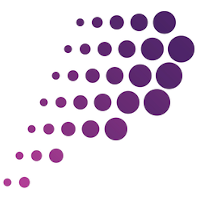
\includegraphics[width=23pt]{./images/pulsepoint.png}}
{PulsePoint}{New York, NY}
{TechOps Intern}{Summer 2017}
\resumeItemListStart
\resumeItem{QPS Monitoring}
{QPS stands for queries per second. Optimized application metric collection/alerting to reduce the false positve rate of QPS drops.}
\resumeItem{System Integrity}
{Automated the backup and data verification of large (\url{~}100GB) databases.}
\resumeItemListEnd

\resumeSubheading
{
\includegraphics[width=23pt]{./images/conceptheca.png}}
{Conceptheca}{Fair Lawn, NJ}
{Mobile Application Developer}{2015 -- 2016}
\resumeItemListStart
\resumeItem{Blood-loss}
{A mobile application on Android/iOS for doctors that calculates the maximum allowable blood-loss that a patient can undergo before reaching critical condition}
\resumeItem{JAM Fractals}
{A mobile game on Android OS that allows a player to mix ingredients to form seemingly random and chaotic fractal images}
\resumeItem{Sepsis Clock}
{An iOS application to help doctors keep track of the time and completion progress of the procedures to treat patients with septic shock}
\resumeItemListEnd
\resumeSubHeadingListEnd
%--------------------------------------

%---------------SKILLS-----------------
\section{Skills}
\resumeSubHeadingListStart
\resumeSubItem{Languages}
{C/C++/Objective-C, Python, Rust, Java, C\#, MATLAB, Verilog, Bash, HTML/CSS, Russian}
\resumeSubItem{Robotics and Sensing Software}{OpenCV, CGAL, ROS, Gazebo}
\resumeSubItem{Robots and Hardware}{Baxter, Xilinx FPGAs, 3D Printing}
\resumeSubItem{Physics Engines}{Bullet, Godot, Unity}
\resumeSubItem{Miscellaneous}{Docker}
\resumeSubHeadingListEnd
%--------------------------------------

%---------------AWARDS-----------------
\section{Awards}
\resumeSubHeadingListStart
\resumeSubItem{2021; Best Paper Award at BigVis}{Graph Cities: Their Buildings, Waves, and Fragments}
\resumeSubItem{2018; HackCooper; $1^{st}$ prize}
{skEye Net - Wireless eye tracking / gaze estimation headset that works in realtime}
\resumeSubItem{2015 --- 2019; Half-tuition scholarship}{Merit scholarship from Cooper Union}
\resumeSubItem{2015 --- 2019; Innovators Merit Scholarship}{Merit scholarship from Cooper Union}
\resumeSubItem{2015; David Lee Memorial Scholarship}{For academic achievment and community service}
\resumeSubHeadingListEnd
%--------------------------------------

\section{Miscellaneous}
\resumeSubHeadingListStart
\resumeSubItem{Peer Reviewes}{2019 - ...}
\resumeItemListStart
\resumeItem{IROS}{Conference on Intelligent Robots and Systems}
\resumeItem{CoRL}{Conference on Robot Learning}
\resumeItem{RSS}{Robotics: Science and Systems Conference}
\resumeItem{RA-L}{IEEE Robotics and Automation Letters}
\resumeItem{BigVis}{Big Data Visual Exploration and Analytics Conference}

\resumeItemListEnd
\resumeSubHeadingListEnd

%------------AFFILIATIONS--------------
% \section{Organizations}
%         \resumeSubHeadingListStart
%                 \resumeSubItem{Rutgers Astronomical Society}
%                 {}
%         \resumeSubHeadingListEnd
%--------------------------------------

\end{document}
